\chapter{GraphQL}
\section{Typ-System}

Das GraphQL-Typ-System wird zur Definierung eines Schemas verwendet.
Ein Schema beschreibt einen GraphQL-Service und besteht aus den abrufbaren Ressourcen, ihren Relationen zueinander und ihren Interaktionsmöglichkeiten.


Eine eingehende Anfrage wird durch die im Schema definierte Datenstruktur validiert.
Wenn die in der Anfrage enthaltene Query durch das Typ-System erfolgreich validiert wurde, wird die beinhaltete Operation an die Implementierung weitergeleitet.
Dafür zerlegt GraphQL die übergebene Query und gibt sie an den jeweiligen Resolver weiter. Diese Resolver interagieren mit der Geschäftslogik und füllen die angeforderten Felder mit Daten.
Die kumulierten Ergebnisse werden als Antwort an den Client zurückgeschickt. 
% \cite[S. 57-58]{kress2020graphql}
% , spec.graphql.org/SchemaDefinition


\section{Schema-Definitions-Sprache SDL}
Da GraphQL laut Spezifikation in jeder beliebigen Sprache implementierbar sein soll wird eine sprachunabhängige Basis für die Definierung des GraphQL-Graphen benötigen.
Diese sprachunabhängige Basis wird durch die in der Spezifikation definierte Beschreibungssprache (\textit{SDL}) gegeben. 
In GraphQL existieren folgende Typ-Definitionen \textit{Skalar, Interface, Object, Input Object, Enum, Union} diese bilden das Rückgrat des Schemas.
Über diese Typen wird in den nachfolgenden Abschnitten eine genauere Übersicht gegeben.

\subsection{Skalare}

Ein Datentyp der nicht mehr weiter vereinfachbar ist wird wie in anderen Programmiersprachen Skalar-Typ genannt.
Skalar-Typen respräsentieren die Blätter, also die primitiven Werte des GraphQL-Typ-Systems. % Kress Seite 60
GraphQL-Antworten entsprechen der Form eines hierarchisch aufgebauten Baumes.
\newline
Grundsätzlich bestehen die Blätter dieses Baumes aus GraphQL-Skalar-Typen (es ist zudem auch möglich, dass die Blätter aus \textit{Null-Werten} oder \textit{Enum-Typen} bestehen).
%spec.graphql.org /ScalarTypeDefinition
GraphQL beinhaltet folgende vordefinierten Skalar-Typen:
\begin{enumerate}
    \item Boolean
    \item Float
    \item Int
    \item String
    \item ID
\end{enumerate}

\begin{JsCode}
    id: Int!
    title: String
\end{JsCode}

Im oben angeführten Codebeispiel werden die Felder \textit{id} und \textit{title} definiert.
Der Name eines Feldes im umgebenden Typ muss dabei eindeutig sein.
Die Deklaration erfolgt mit dem Namen als auch dem Typ des Feldes welche mit einem Doppelpunkt getrennt sind.
Das Feld \textit{id} wird dabei als \textit{not null} deklariert.

\myparagraph{Benutzerdefinierte Skalare}


In den meisten sprachspezifischen Implementierungen ist es möglich eigene Skalar-Typen zu definieren. Diese werden verwendet um beispielsweise verschiedene Datumsformate darzustellen.

\subsection{Enum}

\subsection{Objekt}
Um auf die Blätter des Baumes zuzugreifen werden in GraphQL Objekte als Knoten verwendet.
Diese Objekte halten dabei eine Liste von Feldern die einen bestimmten Wert lieferen.
Dabei kann jedes Feld entweder ein Skalar, Enum, Objekt oder Interface sein.
Laut Spezifikation, sollten Objekte als eine Menge von geordneten Schlüssel-Wert-Paaren serialisiert werden.
Wobei der Name des Feldes der Schlüssel ist und das Ergebnis der Evaluierung des jeweiligen Feldes den Wert abbildet.
Um einen Objekt-Typ zu definieren muss das Schlüsselwort \textit{type} verwendet werden.

\begin{JsCode}
type Book {
    id: Int!
    title: String
    authors: [Author]
}
    
type Author {
    id: Int!
    firstName: String
    lastName: String
    books: [Book]
}
\end{JsCode}

Im oben angeführten Schemaausschnitt werden die beiden Objekte \textit{Author} und \textit{Book} definiert.
Um einen Objekttypen zu definieren wird das Schlüsselwort \textit{type} verwendet.

Das Objekt Book wird dabei mit den Feldern \textit{id, title} und \textit{authors} definiert.
Das Objekt Author erhält die Felder \textit{id, firstName, lastName} und \textit{books}.

Die Felder \textit{id, title, firstName} und \textit{lastName} sind dabei skalare Felder und bilden dabei Blätter des Baumes.
Da zwischen den Objekten Author und Book eine n:m Beziehung besteht, halten beide Objekte eine Liste des jeweils anderen Objekt-Typs.
Listen werden in der SDL wie im obigen Beispiel ersichtlich mit eckigen Klammern definiert.

\subsection{Interface}


\subsection{Input Objekt}


\subsection{Union}

\section{Schema}
Wenn man das Schema als Baumstruktur betrachtet so sind die referenzierten Objekte Verzweigungen des Baumes.
Die Blätter am Ende des Baumes enthalten die eigentlichen Daten.
Die Astverzweigungen sind wichtig, denn sie sind die Referenzen die zu den anderen Objekten verweisen.

Zudem werden die Wurzelknoten der Eingangspunkte der Operationen (Query, Mutation und Subscription) definiert.
Um ein korrektes Schema zu erstellen muss beachtet werden, dass die Typen und Direktiven eindeutig über ihren Namen identifizierbar sind. Außerdem dürfen im Schema definierte Namen nicht mit doppeltem Unterstrich beginnen.
Diese sind für das GraphQL Introspektionsystem reserviert. spec.graphl.org/SchemaDefinition

\section{Wurzel Operationen}
Das Schema definiert die initialen Wurzelknoten der Operationen die es unterstützt (Query, Mutation, Subscription). Dadurch definiert das Schema den Ort im Typ System wo diese Operationen beginnen.
Query ist aber dabei die einzige Operation welche man zwingend definieren muss. Mutations und Subscriptions sind optional und werden, wenn sie nicht explizit definiert werden, nicht unterstützt.
Eine Wurzel-Operation muss dabei ein \textit{Object Type} sein. Desweiteren müssen die Objekttypen der Wurzel-Operationen unterscheiden und dürfen nicht diesselben sein. 


\begin{JsCode}
type Book {
    id: Int!
    title: String
    authors: [Author]
}
    
type Author {
    id: Int!
    firstName: String
    lastName: String
    books: [Book]
}
\end{JsCode}

% Das Objekt Book enthält dabei die Felder id und title. Desweiteren enthält Book eine Liste von Authoren.
% Das Objekt Author enthält die Felder id, firstName und lastName.
% Außerdem enthält Author eine Liste von Büchern die der Autor geschrieben hat.
% Im Beispiel gilt zu beachten, dass eine Ressource mit dem Schlüsselwort \textit{type} versehen ist.
% Zudem sind die Properties der Ressource immer nach dem Schema <name>: <Datentyp> gegliedert.
% Der Datentyp ist dabei entweder ein Objekt, eine Liste von Objekten oder ein skalarer Datentyp.
% Im Schema werden Relationen von Objekten nicht durch eine Schachtelung dieser in einem einzigen Objekt definiert.
Bei komplexeren Graphen würde dies zu einer kaum zu lesenden oder adaptierbaren Schemadefinition führen.
Das Schema besteht somit aus einzelnen, geschlossenen Objekttyp-Definitionen, die einander oder aber ihre Felder referenzieren. Seite 58 und 59
Ist ein Feld mit ! deklariert so darf dieses nicht null sein.

% \section{Typen}
% In GraphQL existieren 6 Typ Definitionen \textit{Skalare, Interfaces, Object, Input Object, Enum, Union} diese bilden das Rückgrat des Schemas.


\section{Parameter}

\section{Querys}

GraphQL erlaubt es den Clients lesend auf die Ressourcen zuzugreifen und genau jene Daten abzufragen welche er benötigt.
Als Ergebnis auf eine Anfrage werden die Daten genau in dem Format zurückgegeben in welcher die Anfrage erfolgt ist.
Dafür bietet GraphQL den Eingangspunkt hinter dem sich das komplette zuvor definierte Graphen Schema befindet.
Um nun auf die Daten zugreifen zu können, muss an den Endpunkt ein in der GraphQL Query Language definiertes Objekt mit den Feldern des Graphen, übergeben werden.
Um nun auf die im Schema definierten Ressourcen lesend zugreifen zu können muss das Schema um Querys erweitert werden. 

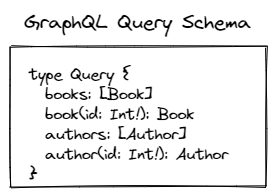
\includegraphics{pics/GraphQL_Query_Schema.png}

\subsection{Designempfehlungen}

placeholder
\pagebreak

\subsection{Verschachtelte Querys}

\subsection{Variablen}

placeholder
\pagebreak

\subsection{Fragmentierung}

\subsection{Aliase}

placeholder
\pagebreak

\section{Mutationen}

\subsection{Designempfehlungen}

placeholder
\pagebreak

\section{Bekannte Probleme}

\subsection{Authentifizierung, Autorisierung und Rollenmanagement}

placeholder
\pagebreak

\subsection{1 + n Problem}

\subsection{Subscriptions}

placeholder
\pagebreak

placeholder
\pagebreak

\subsection{Fehlermanagement}

placeholder
\pagebreak

\subsection{Pagination}

\subsection{Caching}

placeholder
\pagebreak
